\begin{center}
	
\end{center}\chapter{سوخت \lr{LNG}}
\section{کلیات}
گاز طبیعی مایع یا ال‌ان‌جی 
\LTRfootnote{Liquefied Natural Gas}
 به گاز طبیعی‌ای گفته می‌شود که موقتاً برای ذخیره‌سازی یا ترابری در حجم بالا، به حالت مایع تبدیل شده‌است.
 \\
 ال‌ان‌جی، بیشترشامل متان 
 \LTRfootnote{(CH4)} 
 و مقادیر اندکی اتان، پروپان، بوتان و برخی از آلکان‌های سنگین دیگر می‌باشد. البته در مواردی خاص، فرایند پالایش ال‌ان‌جی، می‌تواند به نحوی طراحی شود، که محصول پایانی تولیدشده شامل ۱۰۰ درصد متان باشد. 
 \lr{LNG}
  به عنوان پاک ترین سوخت فسیلی شناخته شده و اقبال به استفاده از این سوخت رو به افزایش است طوری که طبق آمار شناورهای سفارش داده شده برای ساخت در سال 2019، حدود
   17\%  از این شناورها (بر حسب تناژ) از سوخت 
 \lr{LNG} 
   بهره‌مند خواهند شد.
ال‌ان‌جی حجمی معادل یک ششصدم حجم گاز طبیعی در حالت گازی را دارا بوده و محلولی بی‌بو، بی‌رنگ، غیرسمی و غیرخورنده است. این سوخت دارای چگالی کمتری در مقایسه با سوخت‌های رایج بوده و به همین دلیل برای ذخیره سازی نیاز به مخازن بزرگتری دارد.
\begin{figure}[!h]
	\centering
	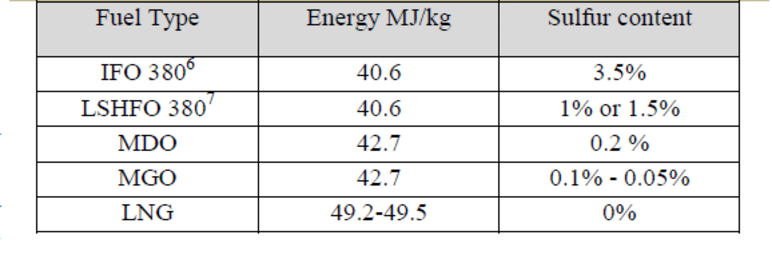
\includegraphics[width=15cm]{Figures/LNG/Fuel Type.png}
	\caption{انواع سوخت}\label{fuel type}
\end{figure}
\newpage
\section{اثرات زیست محیطی و ایمنی}
\subsection{تأثیرات مثبت}
\begin{enumerate}
	\item  کاهش15 تا 20 درصدی انتشار گازهای گلخانه‌ای \lr{(CO2)} به دلیل نسبت بالای هیدروژن به کربن در مقایسه با سایر سوخت‌ها
	\item کاهش 100 درصدی انتشار اکسیدهای گوگرد \lr{(SOx)} در مقایسه با سوخت‌های فعلی
	\item کاهش بالای 90 درصدی انتشار اکسیدهای نیتروژن \lr{(NOx)} در مقایسه با سوخت‌های فعلی
	\item کاهش 100 درصدی انتشار ذرات معلق \lr{(PM)} در مقایسه با سوخت‌های فعلی
\end{enumerate}
\subsection{تأثیرات منفی}
\begin{enumerate}
	\item 	تأثیرات زیست‌محیطی هنگام استخراج، فرآوری، حمل، ذخیره سازی و مصرف نهایی \lr{LNG}
	\item احتمال نشت متان \LTRfootnote{Methane Slip} در موتور شناور به ویژه در فرایندهای احتراق ناقص که بعضا اثرات گلخانه‌ای شدیدتری نسبت به دی اکسید کربن خواهد داشت.
	\item احتمال نشت سوخت مایع در آب دریا و تبخیر منجر به آلودگی هوا

\end{enumerate}

\section{تکنولوژی تولید}
\begin{figure}[!h]
	\centering
	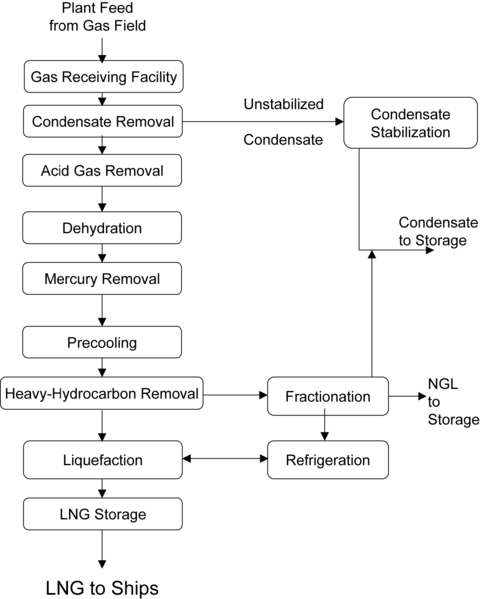
\includegraphics[width=15cm]{Figures/LNG/technology.png}
	\caption{تکنولوژی تولید}\label{technology}
\end{figure}
\subsection{مرحله اول، پیش تصفیه سازی}
ابتدا خوراک گاز طبیعی در واحد زدایش گازهای اسیدی از میان فیلترها عبور نموده و گازهای اسیدی مانند
\lr{CO2} و
\lr{H2S}   
با استفاده از یک محلول آمین اختصاصی در ستون جذب جدا می‌شوند.
سپس واحد آب زدایی گاز طبیعی را تا مقدار مجاز کمتر از 0.1
 \lr{ppm}
  از آب خشک نموده و جریان در ادامه مسیر خود وارد واحد جیوه زدایی می شود. زیرا برای ورود خوراک به واحد مایع سازی باید کمترین میزان جیوه نیز از این ترکیب حذف گردد.
\subsection{مرحله حذف هیدروکربن های سنگین}
پس از یک مرحله خنک سازی ابتدایی با آمونیاک به عنوان مبرد (تا دمای 
8-
 درجه سانتیگراد)، حذف هیدروکربن های سنگین مانند پنتان و بنزن از خوراک گازی صورت می‌گیرد. مقدار مجاز این مواد برای جلوگیری از یخ زدگی خوراک در واحد پایین دستی کمتر از 1 
\lr{ppm}
  است.
\subsection{مرحله مایع سازی}
در این مرحله گاز ورودی توسط سیتم‌های تبرید تحت فشار از دمای 8- درجه سانتی به 162- سانتی گراد خنک گردیده و تبدیل به مایع می شود. در انتها گاز طبیعی مایع شده به مخازن نگهداری ارسال می شود. در بازارهای مصرف، 
\lr{LNG}
 دوباره به حالت گاز در می‌آید. 
\section{تکنولوژی استفاده در کشتی}
\begin{figure}[!h]
	\centering
	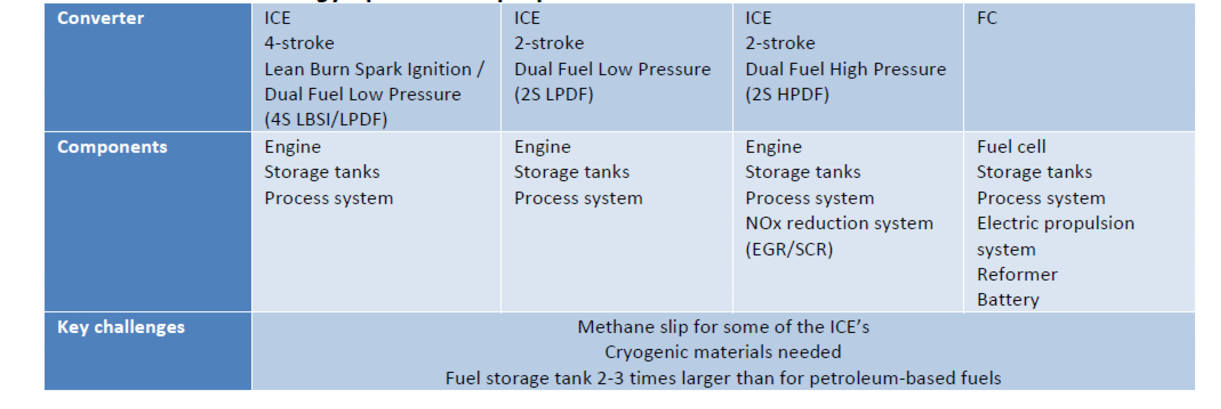
\includegraphics[width=15cm]{Figures/LNG/using in Ship.png}
	\caption{تکنولوژی استفاده در کشتی}\label{using in ship}
\end{figure}
به طور کلی دو گزینه برای استفاده از 
\lr{LNG}
 به عنوان سوخت در کشتی وجود دارد:
 \begin{enumerate}
 	\item استفاده در موتورهای احتراق داخلی \lr{(ICE)}
 	\item استفاده در پیل‌های سوختی  \lr{(Fuel Cell)}
 \end{enumerate}
 به طور کلی سه نوع موتور برای استفاده از 
 \lr{LNG}
  به عنوان سوخت مورد استفاده هستندکه هر سه دوگانه سوز بوده و علاوه بر 
  \lr{LNG}
   از سوخت‌های رایج مانند مازوت هم بهره می‌برند:
    \begin{enumerate}
   	\item موتور دو زمانه فشار پایین
   	\item موتور دو زمانه فشار بالا (با احتمال انتشار \lr{NOx})
   	\item موتور چهارزمانه فشار پایین
   \end{enumerate}
   در ادامه به پیل‌های سوختی پرداخته خواهد شد.
  \subsection{الزامات قانونی}
  علاوه بر قوانین و الزامات محیط زیستی سازمان \lr{IMO} برای کاهش انتشار گازهای گلخانه‌ای \lr{(CO2)}، اکسیدهای گوگرد \lr{(SOx)} واکسید نیتروژن \lr{(NOx)} که می‌تواند میزان گرایش به استفاده از سوخت‌های جایگزین مانند \lr{LNG} را افزایش دهد، الزامات ایمنی کشتی‌های استفاده کننده از سوخت‌های گازی یا سوخت‌های دارای نقطه اشتعال پایین \LTRfootnote{(IGF Code)} به طور مشخص به \lr{LNG} پرداخته و نکات ایمنی برای طراحی و ساخت شناورهای مصرف کننده \lr{LNG} مطرح نموده است. این الزامات شامل سه موضوع اصلی است که عبارتند از:
  \begin{enumerate}
  	\item پیشگیری از نشت سوخت
  	\item پیشگیری از انفجار یا فضای سمی
  	\item مقابله و کاهش اثرات انفجار 
  \end{enumerate}
  الزامات جنبه‌های دیگر مصرف \lr{LNG} به عنوان سوخت دریایی مانند فرایند سوخت رسانی \LTRfootnote{(Bunkering)} هم تا این لحظه به قوانین و مقررات داخلی کشورها واگذار گردیده است.  علاوه بر \lr{IMO} ، اتحادیه اروپا هم الزامات محدودکننده‌ای در راستای کاهش انتشار گازهای گلخانه‌ای و سایر آلاینده‌های هوا وضع نموده است 
\LTRfootnote{(FuelEU Maritime)}.
\section{بررسی اقتصادی \lr{LNG}}
\subsection{قیمت}
	در اکثر نقاط جهان قیمت گاز طبیعی پایین تر از قیمت نفت خام و سوخت‌های سنگین مانند مازوت است. قیمت \lr{LNG} هم ارتباط مستقیمی با قیمت گاز طبیعی دارد که البته هزینه‌های مایع سازی، حمل و نقل و توزیع، ذخیره سازی و سود ذینفعان هم به آن اضافه ‌می‌شود.
در اواسط دهه گذشته میلادی (حدود سال‌های 2015 و 2016) با اکتشاف و بهره‌برداری از منابع جدید گاز طبیعی در امریکا و کاهش قیمت جهانی نفت خام، شاهد کاهش چشمگیر قیمت گاز طبیعی در اکثر نقاط جهان بودیم که طبیعتا کاهش قابل توجه قیمت \lr{LNG} را هم به همراه داشت. از سال 2016 به بعد قیمت \lr{LNG} با شیب ملایمی در حال رشد بوده و پیش بینی می‌شود این روند افزایشی آرام همچنان ادامه دار باشد، هرچند درگیری نظامی روسیه و اوکراین در سال 2022، با ایجاد شوک اقتصادی، باعث افزایش ناگهانی قیمت گاز شد اما با گذشت چند ماه شرایط به یک ثبات نسبی رسید.
در حال حاضر میزان رشد قیمت \lr{LNG} در مقایسه با گازوئیل \lr{(MGO) }و سوخت‌های سنگین کم سولفور کمتر بوده این روند \lr{LNG} را به عنوان یک سوخت با قیمت رقابتی در بازار و یک گزینه مقرون به صرفه در آینده نزدیک مطرح می‌نماید. به ویژه که قوانین زیست محیطی سختگیرانه بعدی هم در راه خواهند بود.
هم اکنون (تابستان 2024) قیمت \lr{LNG} به ثبات نسبی رسیده و اغلب از گازوئیل پایین تر ولی همچنان از سوخت‌هایی مثل مازوت گران تر است اما با توجه به محدودیت‌های زیست محیطی مثل محدودیت سولفور نیم درصد، احتمالا تولید و عرضه مازوت در آینده به صرفه نخواهد بود. 
\subsection{هزینه‌های اولیه}
هزینه‌های اولیه راه‌اندازی سیستم‌های \lr{LNG} بر روی کشتی شامل هزینه موتور، هزینه مخازن و ذخیره سازی، هزینه سیستم‌های آماده سازی و انتقال سوخت و هزینه ارتقا سیستم‌های قبلی می‌شود. در حال حاضر هزینه‌های اولیه سیستم‌های \lr{LNG} (به خصوص به دلیل حجم مخازن بزرگتر و نیاز به عایق بندی به سبب نقطه جوش پایین تر) در مقایسه با سوخت‌های رایج مانند مازوت و گازوئیل بالاتر است اما با توجه افزایش توجهات به سمت \lr{LNG} و همچنین افزایش سرمایه‌گذاری و توسعه فناوری‌های مرتبط، انتظار می‌رود در سال‌های آینده شاهد کاهش نسبی این هزینه‌ها باشیم. در حال حاضر تخمین زده می‌شودکه بااستفاده از سوخت \lr{LNG} در کشتی‌ها، متوسط هزینه‌های اولیه در حدود 20 درصد افزایش پیدا کند. 
\subsection{هزینه‌های ثانویه (عملیاتی)}
در صورتی که قیمت \lr{LNG} در سطح جهانی جهش ناگهانی نداشته باشد، می‌توان هزینه‌های عملیاتی سیستم‌های \lr{LNG} را در مقایسه با سیستم‌های سوخت‌های فعلی، برابر و یا حتی کمتر دانست. چرا که سیستم‌های \lr{LNG} اغلب نیاز به سیستم‌های کاهش انتشار و اسکرابر ندارند و بازدهی و مصرف سوخت موتورهای مصرف کننده \lr{LNG} (دوگانه سوز) تفاوتی با موتورهای قبلی ندارد. همچنین به دلیل پاک تر بودن سوخت \lr{LNG} می‌توان انتظار داشت، هزینه‌های تعمیر و نگهداری موتورها هم در مقایسه با سوخت‌های سنگین کمتر باشد. در ضمن در برخی بنادر به عنوان مشوق تخفیف‌هایی برای شناورهای دارای سوخت \lr{LNG} در نظر می‌گیرند. 
\subsection{میزان تولید، زیرساخت‌ها و میزان دسترسی}
در ابتدای سال 2024، ظرفیت سالانه تولید \lr{LNG}، در حدود 483.1 میلیون تن، تخمین زده می‌شود و با توجه به سرمایه‌گذاری‌های صورت گرفته در نقاط مختلف جهان، انتظار می‌رود این عدد تا سال 2030 به حدود 700 میلیون تن در سال برسد.
همچنین تا پایان سال 2023، 49 ترمینال فعال عرضه کننده سوخت \lr{LNG} دریایی (ساحلی یا فراساحلی) در سراسر جهان در حال خدمت رسانی هستند که مجموع ظرفیت سالانه عرضه سوخت آنها حدود 200 میلیون تن می‌باشد و حداقل 17 ترمینال جدید هم در حال ساخت بوده و به زودی به این ظرفیت اضافه خواهند شد.
اولین بنادری که شروع به عرضه سوخت \lr{LNG} به شناورها نمودند آمستردام و روتردام هلند، فلوریدا امریکا و بنادری در دریای شمال و دریای بالتیک بودند. اما کم کم سایر نقاط جهان مانند بنادر مدیترانه غربی، خلیج مکزیک، سنگاپور، استرالیا، چین، ژاپن، کره جنوبی و حتی بنادر کشورهای خاورمیانه مثل امارات هم سرمایه‌گذاری و بهره برداری از مراکز تامین \lr{LNG} را آغاز نمودند. 
در حال حاضر سوخت \lr{LNG} سهم کمتر از 5 درصدی از بازار سوخت‌های دریایی دارد که احتمالا این عدد در سالهای آینده افزایش قابل توجهی خواهد داشت. با توجه به افزایش روز افزون تولید جهانی \lr{LNG} و روش‌های مختلف توزیع  سوخت در سراسر جهان (حمل دریایی، زمینی و حتی ریلی) می‌توان این گونه فرض کرد که در آینده نزدیک از بابت میزان دسترسی به این سوخت چالش جدی نخواهیم نداشت.
\section{وضعیت ایران}
\subsection{تاریخچه تولید \lr{LNG} در ایران}
ایران با دارا بودن دومین ذخایر بزرگ گاز طبیعی جهان، پتانسیل قابل توجهی برای تبدیل شدن به یک بازیگر کلیدی در بازار \lr{LNG} جهانی را دارد. با این حال، ایران تاکنون در تولید \lr{LNG} موفقیت چندانی کسب نکرده است.
\begin{enumerate}
	\item دهه 1970: اولین مطالعات برای احداث واحدهای \lr{LNG} در ایران انجام شد.
	\item دهه 1990: به دلیل تحریم‌ها و عدم ثبات سیاسی، پیشرفت‌ها متوقف شد.
	\item دهه 2000: چندین پروژه \lr{LNG} با مشارکت شرکت‌های خارجی آغاز شد، اما هیچکدام به بهره‌برداری نرسیدند.
	\item دهه 2010: ایران به دنبال توسعه مجدد پروژه‌های \lr{LNG} با تمرکز بر فناوری‌های کوچک مقیاس است.
\end{enumerate}
ایران در حال ساخت یک کارخانه تولید \lr{LNG} با ظرفیت 1.5 میلیون تن در سال در عسلویه است. این کارخانه توسط یک شرکت ایرانی با هدف افزایش مصارف داخلی و همچنین صادرات احداث گردیده است. فاز اول این کارخانه شامل نیروگاه 1100 مگاواتی، مخازن ذخیره‌سازی \lr{LNG} و \lr{LPG}، و اسکله‌های دریایی است. 
ایران برای تولید \lr{LNG} به فناوری پیشرفته ای نیاز دارد که ممکن است به دلیل تحریم ها در دسترس نباشد. ساخت واحدهای \lr{LNG} نیاز به سرمایه گذاری عظیمی دارد. تحریم های بانکی و اقتصادی ایران تامین مالی پروژه‌های \lr{LNG} را با مشکل مواجه می کند. ایران با رقابت شدیدی در بازار \lr{LNG} از دیگر کشورها مانند قطر، استرالیا و ایالات متحده مواجه است.
با افزایش تولید \lr{LNG} در کشور، امکان عرضه آن به عنوان سوخت دریایی در بنادر ایران فراهم خواهد شد.

$\pd{s}{d}$
\subsection{پیش بینی تقریبی از آینده}
پیش بینی ها نشان می‌دهند که گاز طبیعی مایع \lr{(LNG)} تا سال ۲۰۳۰ به عنوان یک سوخت به صرفه در صنعت حمل و نقل دریایی باقی خواهد ماند. در حال حاضر، \lr{LNG}  حدود 6.4 درصد از سوخت های مورد نیاز صنعت کشتیرانی را تأمین میکند و انتظار میرود که این میزان تا سال ۲۰۳۰ به ۱۰.۷ درصد افزایش یابد.
همچنین، با توجه به قوانین سختگیرانه سازمان بین المللی دریانوردی \lr{(IMO)} برای کاهش انتشار گازهای     گلخانه ای، استفاده از \lr{LNG} به عنوان یک سوخت پاک و پایدار تشویق خواهد شد.
در آینده، با توسعه زیرساخت های ذخیره سازی و سوخت رسانی \lr{LNG}، تعداد کشتیهایی که از این سوخت استفاده میکنند به طور قابل توجهی افزایش خواهد یافت. پیش بینی میشود که بیش از ۱۰۰۰ فروند کشتی با سوخت \lr{LNG} تا سال ۲۰۲۷ در آبهای بین المللی فعالیت کنند.
\section{نتیجه‌گیری}
\begin{figure}[!h]
	\centering
	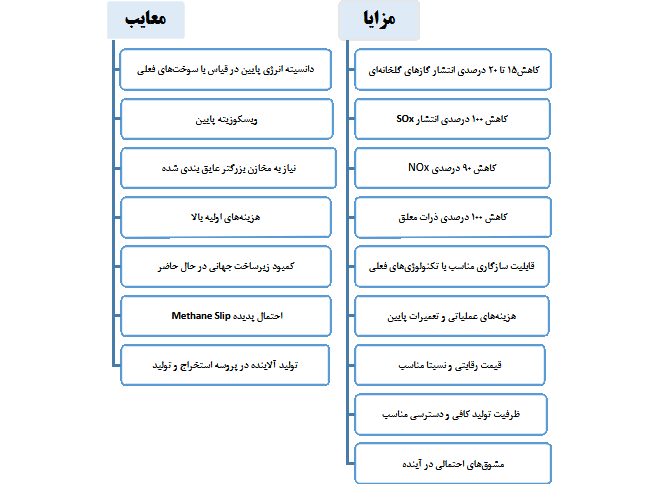
\includegraphics[width=20cm]{Figures/LNG/conv.png}
	\caption{جمع بندی}\label{conv}
\end{figure}



